\documentclass[landscape,11pt]{article}
\usepackage[UTF8]{ctex}
\usepackage{geometry}
\geometry{margin=0.7cm}
\usepackage{tikz}
\usetikzlibrary{arrows.meta, positioning, fit, backgrounds, calc, shadows, shapes.geometric}
\usepackage{xcolor}
\usepackage{booktabs}
\usepackage{amsmath}
\usepackage{fontspec}

% --- Color scheme (customize for your project) ---
\definecolor{mainblue}{RGB}{34,80,140}
\definecolor{wingreen}{RGB}{50,140,50}
\definecolor{secondaryblue}{RGB}{34,101,156}
\definecolor{accent}{RGB}{200,40,40}
\definecolor{accentorange}{RGB}{210,120,20}
\definecolor{lightbg}{RGB}{245,248,252}

% --- TikZ component styles ---
\tikzset{
  comp/.style={draw=black!70, thick, rounded corners=4pt, fill=white,
               minimum width=2.0cm, minimum height=0.7cm, align=center,
               font=\footnotesize\bfseries,
               drop shadow={shadow xshift=0.6pt, shadow yshift=-0.6pt, opacity=0.08}},
  sbox/.style={draw=black!40, thick, rounded corners=6pt, inner sep=8pt},
  arrow/.style={->, >=Stealth, thick, black!60},
  tag/.style={font=\scriptsize\bfseries, rounded corners=2pt, inner sep=2pt, text=white},
}

\begin{document}
\thispagestyle{empty}

% ============================================================
% Page 1: Example — System Architecture Diagram
% ============================================================

\begin{center}
{\LARGE\bfseries\textcolor{mainblue}{Project Title}}\\[3pt]
{\large\textcolor{black!50}{Subtitle $\;\cdot\;$ Keywords}}
\end{center}

\vspace{4pt}

\begin{center}
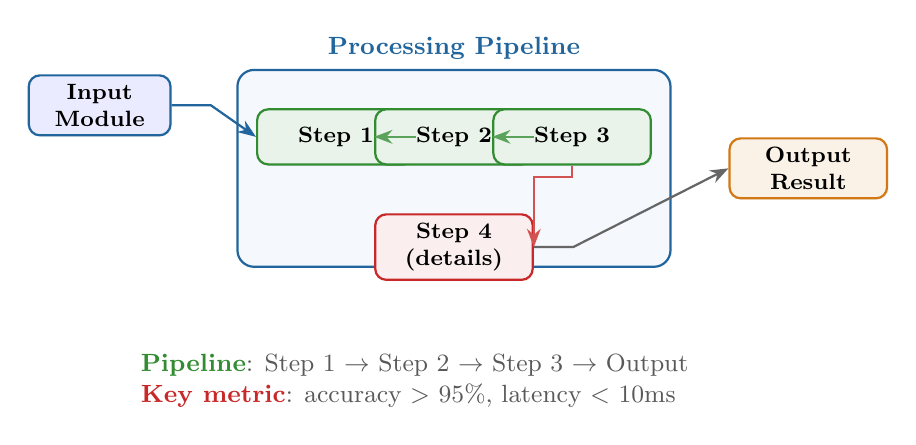
\begin{tikzpicture}[node distance=0.4cm and 0.5cm]

% --- Example: Input module ---
\node[comp, fill=blue!8, draw=secondaryblue, minimum width=1.8cm] (input) at (-6, 0)
    {Input\\Module};

% --- Example: Processing group ---
\node[sbox, fill=lightbg, draw=secondaryblue, minimum width=5.5cm, minimum height=2.5cm,
      label={[font=\small\bfseries, secondaryblue]above:Processing Pipeline}]
      (pipeline) at (-1.5, -0.8) {};

\node[comp, fill=wingreen!10, draw=wingreen] (step1) at (-3.0, -0.4) {Step 1};
\node[comp, fill=wingreen!10, draw=wingreen] (step2) at (-1.5, -0.4) {Step 2};
\node[comp, fill=wingreen!10, draw=wingreen] (step3) at (0.0, -0.4) {Step 3};

\node[comp, fill=accent!8, draw=accent] (step4) at (-1.5, -1.8) {Step 4\\(details)};

\draw[arrow, wingreen!80] (step1) -- (step2);
\draw[arrow, wingreen!80] (step2) -- (step3);
\draw[arrow, accent!80]   (step3.south) -- ++(0, -0.15) -| (step4.east);

\draw[arrow, secondaryblue] (input.east) -- ++(0.5, 0) -- (step1.west);

% --- Example: Output ---
\node[comp, fill=accentorange!10, draw=accentorange, minimum width=2.0cm] (output)
    at (3.0, -0.8) {Output\\Result};

\draw[arrow] (step4.east) -- ++(0.5, 0) -- (output.west);

% --- Annotations (bottom-left) ---
\node[font=\small, align=left, text=black!65] at (-2.0, -3.5) {%
    \textcolor{wingreen}{\textbf{Pipeline}}: Step 1 $\to$ Step 2 $\to$ Step 3 $\to$ Output\\
    \textcolor{accent}{\textbf{Key metric}}: accuracy $>$ 95\%, latency $<$ 10ms
};

\end{tikzpicture}
\end{center}

\newpage
\thispagestyle{empty}

% ============================================================
% Page 2: Example — Module Details + Table
% ============================================================

\begin{center}
{\LARGE\bfseries\textcolor{mainblue}{Module Deep Dive}}\\[3pt]
{\large\textcolor{black!50}{Architecture $\;\cdot\;$ Parameters $\;\cdot\;$ Results}}
\end{center}

\vspace{6pt}

\begin{minipage}[t]{0.48\textwidth}

{\normalsize\bfseries\textcolor{mainblue}{Architecture}}

\vspace{4pt}

\begin{center}
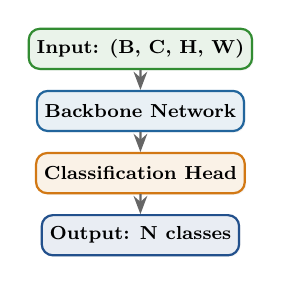
\begin{tikzpicture}[node distance=0.3cm, scale=0.85, transform shape]
  \node[comp, fill=wingreen!10, draw=wingreen, minimum width=2.8cm, minimum height=0.6cm]
      (a) at (0, 0) {Input: (B, C, H, W)};
  \node[comp, fill=secondaryblue!10, draw=secondaryblue, minimum width=2.8cm, minimum height=0.6cm,
        below=of a] (b) {Backbone Network};
  \node[comp, fill=accentorange!10, draw=accentorange, minimum width=2.8cm, minimum height=0.6cm,
        below=of b] (c) {Classification Head};
  \node[comp, fill=mainblue!10, draw=mainblue, minimum width=2.8cm, minimum height=0.6cm,
        below=of c] (d) {Output: N classes};

  \draw[arrow, thick] (a) -- (b);
  \draw[arrow, thick] (b) -- (c);
  \draw[arrow, thick] (c) -- (d);
\end{tikzpicture}
\end{center}

\end{minipage}
\hfill
\begin{minipage}[t]{0.48\textwidth}

{\normalsize\bfseries\textcolor{mainblue}{Key Parameters}}

\vspace{4pt}

\begin{tabular}{ll}
\toprule
\textbf{Parameter} & \textbf{Value} \\
\midrule
Input size      & 224 $\times$ 224 \\
Batch size      & 32 \\
Learning rate   & 1e-4 \\
Optimizer       & AdamW \\
Epochs          & 100 \\
\bottomrule
\end{tabular}

\vspace{8pt}

{\normalsize\bfseries\textcolor{mainblue}{Results}}

\vspace{4pt}

\begin{tabular}{lc}
\toprule
\textbf{Metric} & \textbf{Score} \\
\midrule
Accuracy  & 95.2\% \\
F1 Score  & 0.93  \\
Latency   & 8ms   \\
\bottomrule
\end{tabular}

\end{minipage}

\end{document}
